\pdfbookmark{Общая характеристика работы}{characteristic}             % Закладка pdf
\section*{Общая характеристика работы}

\newcommand{\actuality}{\pdfbookmark[1]{Актуальность темы исследования}{actuality}\underline{\textbf{\actualityTXT}}}

\newcommand{\progress}{\pdfbookmark[1]{Степень разработанности темы исследования}{progress}\underline{\textbf{\progressTXT}}}

\newcommand{\aim}{\pdfbookmark[1]{Цели}{aim}\underline{{\textbf\aimTXT}}}
\newcommand{\tasks}{\pdfbookmark[1]{Задачи}{tasks}\underline{\textbf{\tasksTXT}}}
\newcommand{\aimtasks}{\pdfbookmark[1]{Цели и задачи}{aimtasks}\aimtasksTXT}
\newcommand{\novelty}{\pdfbookmark[1]{Научная новизна}{novelty}\underline{\textbf{\noveltyTXT}}}
\newcommand{\influence}{\pdfbookmark[1]{Теоретическая и практическая значимость работы}{influence}\underline{\textbf{\influenceTXT}}}
\newcommand{\methods}{\pdfbookmark[1]{Методология и методы исследования}{methods}\underline{\textbf{\methodsTXT}}}
\newcommand{\defpositions}{\pdfbookmark[1]{Положения, выносимые на защиту}{defpositions}\underline{\textbf{\defpositionsTXT}}}
\newcommand{\reliability}{\pdfbookmark[1]{Достоверность}{reliability}\underline{\textbf{\reliabilityTXT}}}
\newcommand{\contribution}{\pdfbookmark[1]{Личный вклад}{contribution}\underline{\textbf{\contributionTXT}}}
\newcommand{\publications}{\pdfbookmark[1]{Публикации}{publications}\underline{\textbf{\publicationsTXT}}}


{\actuality}
В современном мире становится всё больше данных, которые требуют обработки и анализа. При этом графы являются одной из самых распространённых и удобных структур, позволяя компактно представлять большие объёмы информации и реализовывать эффективные алгоритмы для её анализа. Графы используются в статическом анализе программ~\cite{rehof2001type,zheng2008demand} и биоинформатике~\cite{sevon2008subgraph}, в социальных сетях~\cite{socialgraph}, сетевом анализе~\cite{zhang2016context} и т.д. Также в настоящее время активно развиваются графовые базы данных, используемые для хранения данных в виде графов и реализации запросов к ним. Следует упомянуть такие графовые базы данных, как RedisGraph$\footnote{Графовая база данных RedisGraph: https://oss.redislabs.com/redisgraph/ (дата обращения: 14.01.2022).}$ и Neo4j$\footnote{Графовая база данных Neo4j: https://neo4j.com/ (дата обращения: 14.01.2022).}$. %HyperGraphDB и OrientDB.

Одной из важнейших задач анализа графов является поиск путей. Имеются разные вариации этой задачи: непосредственный поиск определённых путей, задача достижимости (сами пути не ищутся, но доказывается их существование) и т.д.


В рамках этих задач могут задаваться специальные свойства искомых путей. Одним из способов описания таких свойств является использование формального языка над некоторым алфавитом~\cite{barrett2000formal}. Таким способом можно ограничить множество слов, получаемых конкатенацией меток на дугах рассматриваемых путей. Таким образом, в задачах поиска путей в помеченном графе с заданным формальным языком рассматриваются только те пути, которые образуют слова, принадлежащие этому языку. В настоящее время активно исследуются ограничения, представленные в виде контекстно-свободных (КС) языков~\cite{rehof2001type,reps1998program,bradford2017efficient,hellings2014conjunctive,hellings2020explaining}. Такие языки позволяют описывать более широкий набор ограничений, чем активно используемые на практике регулярные выражения~\cite{koschmieder2012regular,calvanese2000answering}.

С практической точки зрения, одним из распространённых способов получения высокопроизводительных реализаций алгоритмов анализа графов является использование методов линейной алгебры~\cite{kepner2011graph}. При этом существующие алгоритмы, фактически, переводятся на язык линейной алгебры, т.е. для представления графа используются разреженные матрицы (такие матрицы, которые имеют малое количество ненулевых элементов), а для анализа и преобразований графа используются операции над матрицами (умножение матриц, сложение, транспонирование матриц и т.д.). Например, давно известны такие представления графа, как матрица смежности или матрица инцидентности, а такому преобразованию ориентированного графа, как инвертирование направлений дуг соответствует операция транспонирования матрицы смежности. Для тех алгоритмов анализа графов, которые позволяют такой <<перевод>>, становится возможным  использовать параллельные вычисления, в частности, на основе GPU-технологий, что позволяет существенно улучшить их производительность. Кроме того, такого рода алгоритмы зачастую просты в реализации, так как позволяют использовать существующие библиотеки линейной алгебры (SuiteSparse:GraphBLAS$\footnote{SuiteSparse:GraphBLAS~--- реализация стандарта GraphBLAS на языке \texttt{C}: https://github.com/DrTimothyAldenDavis/GraphBLAS (дата обращения: 14.01.2022).}$, cuSPARSE$\footnote{Библиотека линейной алгебры cuSPARSE, используемая для работы с разреженными матрицами на GPU: https://docs.nvidia.com/cuda/cusparse/index.html (дата обращения: 14.01.2022).}$, cuBLAS$\footnote{Библиотека линейной алгебры cuBLAS на основе GPU-технологий: https://docs.nvidia.com/cuda/cublas/index.html (дата обращения: 14.01.2022).}$, cuBool$\footnote{Библиотека булевой линейной алгебры cuBool, использумая для работы с булевыми разреженными матрицами и векторами на GPU: https://github.com/JetBrains-Research/cuBool (дата обращения: 14.01.2022).}$, m4ri$\footnote{m4ri~--- библиотека для быстрой арифметики с плотными булевыми матрицами: https://github.com/malb/m4ri (дата обращения: 14.01.2022).}$, Scipy$\footnote{Scipy~--- библиотека для языка программирования \texttt{Python} с открытым исходным кодом, предназначенная для выполнения научных и инженерных расчётов: https://scipy.org/ (дата обращения: 14.01.2022).}$ и др.).

Однако возможность использования методов линейной алгебры в задачах поиска путей в графе с заданными КС-ограничениями в настоящее время не исследована. Как показывает практика, существующие решения данной задачи страдают от недостаточной производительности и не справляются с постоянно растущими размерами реальных графов~\cite{kuijpers2019experimental}. В то же время создание новых решений, использующих методы линейной алгебры, позволит решить данную проблему с помощью теоретических и практических достижений линейной алгебры.

{\progress}
В последнее время появилось значительное число работ, посвященных классическим алгоритмам анализа графов, переведённых на язык линейной алгебры. Например, Айдын Булук (Aydin Bulu\c{c}), 
Упасана Шридхар (Upasana Sridhar), Питер Чжан (Peter Zhang), Арифул Азад (Ariful Azad) и Лейуань Ван (Leyuan Wang) в своих работах~\cite{bulucc2011parallel,sridhar2019delta,zhang2016gbtl,azad2015parallel,wang2016comparative} показывают применимость на практике алгебраических версий таких алгоритмов, как поиск в ширину, алгоритм Дейкстры, алгоритм Беллмана-Форда, алгоритм поиска наибольшего паросочетания в двудольном графе и алгоритм подсчёта количества треугольников в графе.

На фоне роста популярности идеи решения задач анализа графов с помощью методов линейной алгебры относительно недавно был создан стандарт GraphBLAS~\cite{graphblas}, который определяет базовые <<строительные блоки>> алгоритмов анализа графов в терминах линейной алгебры. Такими <<блоками>>, например, являются умножение и другие операции над матрицами, так как стандарт GraphBLAS использует представление графов в виде матриц смежности. Также, ввиду того, что данные на практике разрежены, целесообразно использовать разреженный формат для этих матриц. Стоит отметить, что не каждый алгоритм анализа графов можно переформулировать на языке линейной алгебры. Так, например, до сих пор это не сделано для алгоритма обхода произвольного графа, использующего поиск в глубину~\cite{spampinato2019linear}. Также в настоящее время это не сделано и для алгоритмов поиска путей в графе с заданными КС-ограничениями.

Задача поиска путей в графе с заданными КС-ограничениями является одной из важных задач анализа графов. Её частным случаем является задача синтаксического анализа КС-языков, в которой анализируются строки, что эквивалентно анализу только линейно-помеченных графов. Лесли Вэлиант (Leslie Valiant) провёл исследование~\cite{valiant1975general}, посвященное синтаксическому анализу КС-языков с использованием операций над матрицами. Предложенный им субкубический алгоритм для заданных строки и КС-грамматики определяет порождается ли эта строка заданной грамматикой с помощью операций умножения булевых матриц. Впервые вопрос о возможности нахождения матричного алгоритма поиска путей в графе с заданными КС-ограничениями исследовал Михалис Яннакакис (Mihalis Yannakakis)~\cite{yannakakis1990graph}. Он указывал, что алгоритм Вэлианта может быть расширен для анализа графов без циклов, но сомневался в возможности создания субкубического алгоритма для анализа произвольных графов. 

Однако для частного случая КС-ограничений существует алгоритм поиска путей в графе, сформулированный на языке линейной алгебры. Такой алгоритм был предложен Филипом Брэдфордом (Philip Bradford)~\cite{bradford2017efficient}, исследовавшим задачу достижимости в графе с заданными КС-ограничениями. 

Кроме того, существует ряд работ~\cite{hellings2014conjunctive,medeiros2018efficient,santos2018bottom,grigorev2017context}, посвященных задаче поиска путей в произвольном графе с заданными произвольными КС-ограничениями и основанных на различных алгоритмах синтаксического анализа (LR, LL, GLL, CYK). Среди них работы Семёна Григорьева, Джелле Хеллингса (Jelle Hellings), Чиро Медейроса (Ciro Medeiros) и Мартина Мюзиканте (Martin Musicante). Стоит отметить, что большинство из представленных алгоритмов требуют представить КС-ограничения на пути в графе в виде КС-грамматики в некоторой нормальной форме. Отдельный интерес представляют собой алгоритмы, не требующие дополнительных преобразований структур, описывающих входные КС-ограничения, так как почти любое такое преобразование обычно приводит к увеличению размеров этих структур, что может негативно сказаться на производительности. Кроме того, после таких преобразований могут возникнуть сложности с интерпретацией результатов анализа графа в терминах изначальной структуры, заданной пользователем. Примерами алгоритмов поиска путей в графе с заданными КС-ограничениями, не требующих преобразований входной КС-грамматики, являются алгоритмы~\cite{medeiros2018efficient,grigorev2017context}, основанные на алгоритмах синтаксического анализа LL и GLL.

Таким образом, на текущий момент не существует алгоритма поиска путей в произвольном графе с заданными произвольными КС-ограничениями, выраженного на языке линейной алгебры. Поэтому необходимо исследовать возможность разработки таких алгоритмов.
%Этот раздел должен быть отдельным структурным элементом по
% ГОСТ, но он, как правило, включается в описание актуальности
% темы. Нужен он отдельным структурынм элемементом или нет ---
% смотрите другие диссертации вашего совета, скорее всего не нужен.

{\aim} данной работы является исследование применимости методов линейной алгебры к задаче поиска путей в графе с заданными КС-ограничениями для получения высокопроизводительных реализаций на основе параллельных вычислений.

Достижение поставленной цели обеспечивается решением следующих {\tasks}.
\begin{enumerate}[beginpenalty=10000] % https://tex.stackexchange.com/a/476052/104425
  \item Разработать подход к поиску путей в графе с КС-ограничениями на основе методов линейной алгебры.
  \item Разработать алгоритм, использующий предложенный подход и решающий задачи поиска путей в графе с заданными КС-ограничениями.
  \item Разработать алгоритм поиска путей в графе с заданными КС-ограничениями, использующий предложенный подход и не требующий преобразования входной КС-грамматики.
  \item Реализовать предложенные алгоритмы с использованием параллельных вычислений, провести их экспериментальное исследование на реальных данных, сравнить их с существующими реализациями, а также между собой.
\end{enumerate}


{\influence} 
Теоретическая значимость диссертационного исследования заключается в разработке подхода к поиску путей в графе с заданными КС-ограничениями, использующего методы линейной алгебры, в разработке формальных алгоритмов, использующих полученный подход, а также в формальном доказательстве завершаемости, корректности и оценок временной сложности разработанных алгоритмов.

В ходе исследования предложенные алгоритмы реализованы с использованием параллельных вычислений, что позволило ускорить время анализа графов до 3 порядков и уменьшить объём потребляемой памяти до 2 порядков по сравнению с существующими реализациями. Кроме того, выполненные реализации могут быть интегрированы с такими графовыми базами данных, как RedisGraph. Это позволит расширить языки запросов к этим базам данных.

{\methods} Методология исследования основана на линейной алгебре и теории графов. В работе использован стандарт GraphBLAS, объединяющий теорию графов и линейную алгебру. Кроме того, в исследовании использовалась теория формальных языков, а также теория сложности. Наконец, для реализации алгоритмов использовались CPU и GPU-технологии. %Одной из задач, для которых до сих пор не найдена формулировка в терминах линейной алгебры, является поиск путей в графе с ограничениями в виде КС-грамматик. Данная задача использует подход к анализу строк, который начал активно развиваться в 50-х годах 20-го века в связи с изучением естественных языков (работы Н.~Хомского). В последствии этот подход получил широкое распространение в различных областях, в том числе и связанных с анализом графов.
%При этом основными элементами данного подхода являются алфавит и грамматика исследуемого языка, выступающего в качестве ограничения на искомые пути в графе. Решаемые в связи с этим задачи связаны с поиском эффективных алгоритмов нахождения путей, удовлетворяющих заданным ограничениям.

{\defpositions}
\begin{enumerate}[beginpenalty=10000] % https://tex.stackexchange.com/a/476052/104425
	\item Разработан подход к поиску путей в графе с заданными КС-ограничениями на основе методов линейной алгебры, который позволяет использовать теоретические и практические достижения линейной алгебры для решения данной задачи.
	\item Разработан алгоритм, использующий предложенный подход и решающий задачи поиска путей в графе с заданными КС-ограничениями. Доказана завершаемость и корректность предложенного алгоритма. Получена теоретическая оценка сверху временной сложности алгоритма. Предложенный алгоритм использует операции над матрицами, которые позволяют применять широкий класс оптимизаций и дают возможность автоматически распараллеливать вычисления за счёт существующих библиотек линейной алгебры.
	\item Разработан алгоритм поиска путей в графе с заданными КС-ограничениями, использующий предложенный подход и не требующий преобразования входной КС-грамматики. Доказана завершаемость и корректность предложенного алгоритма. Получена теоретическая оценка сверху временной сложности алгоритма. Предложенный алгоритм позволяет работать с произвольными входными КС-грамматиками без необходимости их преобразования, что позволяет избежать значительного увеличения размеров входной грамматики и увлечения времени работы алгоритма.
	\item Предложенные алгоритмы реализованы с использованием параллельных вычислений. Проведено экспериментальное исследование разработанных алгоритмов на реальных RDF данных и графах, построенных для статического анализа программ. Было проведено сравнение полученных реализаций между собой, с существующими решениями из области статического анализа и с решениями, основанными на различных алгоритмах синтаксического анализа. Результаты сравнения показывают, что предложенные реализации для задачи достижимости позволяют ускорить время анализа до 2 порядков и потребляют до 2 раз меньше памяти по сравнению с существующими решениями, а для задач поиска одного и поиска всех путей в графе позволяют ускорить время анализа до 3 порядков и до 2 порядков снизить потребление памяти.
\end{enumerate}

{\novelty.}
\begin{enumerate}[beginpenalty=10000] % https://tex.stackexchange.com/a/476052/104425
	
	\item Предложен новый подход к поиску путей в графе с заданными КС-ограничениями, который позволяет использовать теоретические и практические аспекты линейной алгебры для решения задачи поиска путей в графе с КС-ограничениями. 
	
	\item Впервые получен алгоритм поиска путей в произвольном графе с заданными произвольными КС-ограничениями, сформулированный в терминах линейной алгебры, что позволяет применять в этом алгоритме широкий класс оптимизаций для вычисления операций над матрицами, распараллеливать вычисления и существенно улучшить производительность.
	
	\item В диссертации также предложен алгоритм поиска путей в графе с заданными КС-ограничениями, сформулированный в терминах линейной алгебры и не требующий преобразования входной КС-грамматики, в отличие от алгоритмов, предложенных в работах Семёна Григорьева, Джелле Хеллингса и Филиппа Брэдфорда. Таким образом, предложенный в диссертации алгоритм позволяет избежать значительного увеличения размера входной грамматики, от которого напрямую зависит время его работы.
	
	%\item Экспериментальное исследование алгоритмов поиска путей в произвольном графе с заданными произвольными КС-ограничениями, использующих операции линейной алгебры проводится впервые и позволяет судить о применимости на практике разработанных алгоритмов.
	
\end{enumerate}

{\reliability} 
Достоверность и обоснованность результатов исследования опирается на использовании формальных методов доказательств  и инженерные эксперименты.

Основные результаты работы были представлены на ряде международных научных конференций: Joint Workshop on Graph Data Management Experiences \& Systems (GRADES) and Network Data Analytics (NDA) (совместно с конференцией SIGMOD) 2018 (Хьюстон, Техас, США), 2020 (Портленд, Орегон, США) и 2021 (Сиань, Шэньси, Китай); 24th European Conference on Advances in Databases and Information Systems (ADBIS) 2020 (Лион, Франция); VLDB PhD Workshop совместно с 47th International Conference on Very Large Data Bases 2021 (Копенгаген, Дания). Также исследование было поддержано грантом РНФ \textnumero 18-11-00100 и грантом РФФИ \textnumero 19-37-90101.

%{\contribution} Автор принимал активное участие \ldots

{\publications} Все результаты диссертации изложены в 8 научных работах~\cite{azimov1,azimov2,azimov3,azimov4,azimov5,azimov6,azimov7,azimov8}. Из них 3 работы~\cite{azimov6,azimov7,azimov8} опубликованы в журналах из <<Перечня российских рецензируемых научных журналов, в которых должны быть опубликованы основные научные результаты диссертаций на соискание ученых степеней доктора и кандидата наук>>, рекомендовано ВАК. 5 работ~\cite{azimov1,azimov2,azimov3,azimov4,azimov5} индексируются в базе данных Scopus. Работы~\cite{azimov1,azimov2,azimov3,azimov4,azimov6,azimov7,azimov8} написаны в соавторстве. В работе~\cite{azimov1} автору принадлежит разработка и реализация алгоритма, решающего задачу достижимости в графе с заданными КС-ограничениями с использованием методов линейной алгебры, доказательство корректности разработанного алгоритма, постановка экспериментов; соавторы участвовали в обсуждении основных идей статьи, выполняли обзор предметной области. В работе~\cite{azimov2} автору принадлежит разработка и реализация алгоритма, решающего задачу поиска одного пути в графе с заданными КС-ограничениями с использованием методов линейной алгебры, доказательство корректности разработанного алгоритма; соавторы проводили экспериментальное исследование, участвовали в формализации и улучшении изложения идей статьи. В работе~\cite{azimov3} вклад автора заключается в доказательстве корректности алгоритма поиска путей в графе с заданными КС-ограничениями, не требующего преобразований входной КС-грамматики, а также в работе над текстом; соавторам принадлежит идея алгоритма и постановка экспериментов. В работе~\cite{azimov4} автору принадлежит разработка и реализация алгоритма, решающего задачу поиска всех путей в графе с заданными КС-ограничениями с использованием методов линейной алгебры, доказательство корректности разработанного алгоритма, работа над текстом; соавторы проводили экспериментальное исследование. В работах~\cite{azimov6,azimov7} вклад автора заключается в разработке и реализации алгоритма, решающего задачу достижимости в графе с заданными ограничениями в виде конъюнктивных языков, доказательстве корректности разработанного алгоритма и постановке экспериментов; соавторы участвовали в обсуждении основных идей статьи и выполняли обзор предметной области. В работе~\cite{azimov8} автору принадлежит разработка и реализация алгоритма, решающего задачу поиска всех путей в графе с заданными КС-ограничениями с использованием матриц с множествами промежуточных вершин, а также работа над текстом; соавторы проводили экспериментальное исследование.

\paragraph{Благодарности.} Прежде всего я бы хотел поблагодарить своего научного руководителя, Семёна Вячеславовича Григорьева, за руководство на всех этапах данного исследования, за готовность поддержать и поделиться своим опытом и за неоценимый вклад в мою работу. Также хочу поблагодарить Дмитрия Владимировича Кознова за его мудрость, активное участие и за многочисленные беседы о моей диссертации, которые оказали огромное влияние на мою работу и на меня в целом.

Я выражаю благодарность Андрею Николаевичу Терехову и кафедре системного программирования СПбГУ, а также Дмитрию Юрьевичу Булычеву, Андрею Владимировичу Иванову и компаниям JetBrains и Huawei за уникальную возможность заниматься наукой как основной деятельностью.

Я благодарен Владимиру Александровичу Кутуеву и Владе Владимировне Погожельской за помощь в постановке экспериментов.

Отдельную благодарность хочется выразить моей жене, Светлане Дмитриевне Азимовой, и моему сыну, Артёму Рустамовичу Азимову, за вдохновение, любовь и поддержку, ведь они занимают все мои мысли и всё моё сердце, и всё в этой жизни я делаю именно ради них. Также я хочу поблагодарить моего брата, Тимура Шухратулловича Азимова, за разделение моих интересов и поддержку. Наконец, я благодарен моим дорогим родителям, Шухратулло Сулханкуловичу и Елене Ивановне Азимовым, которые являются моей опорой на протяжении всей жизни и сделали меня тем, кто я есть сейчас.
 % Характеристика работы по структуре во введении и в автореферате не отличается (ГОСТ Р 7.0.11, пункты 5.3.1 и 9.2.1), потому её загружаем из одного и того же внешнего файла, предварительно задав форму выделения некоторым параметрам

%Диссертационная работа была выполнена при поддержке грантов \dots

%\underline{\textbf{Объем и структура работы.}} Диссертация состоит из~введения,
%четырех глав, заключения и~приложения. Полный объем диссертации
%\textbf{ХХХ}~страниц текста с~\textbf{ХХ}~рисунками и~5~таблицами. Список
%литературы содержит \textbf{ХХX}~наименование.

\pdfbookmark{Содержание работы}{description}                          % Закладка pdf
\section*{Содержание работы}
Во \underline{\textbf{введении}} обосновывается актуальность
исследований, проводимых в~рамках данной диссертационной работы,
приводится краткий обзор научной литературы по~изучаемой проблеме,
формулируется цель, ставятся задачи работы, излагается научная новизна
и практическая значимость представляемой работы.


\underline{\textbf{Первая глава}} посвящена обзору области исследования. Вводятся основные термины и определения, используемые в работе: основные понятия и методы линейной алгебры, теории графов, теории формальных языков. Вводится формальная постановка задач достижимости, поиска одного пути и поиска всех путей в графе с заданными КС-ограничениями.

Даётся краткий обзор основных алгоритмов поиска путей в графе с заданными КС-ограничениями, которые основаны на различных методах синтаксического анализа: на основе (G)LL и (G)LR алгоритмов, на основе CYK алгоритма, с использованием парсер-комбинаторов.

Рассматриваются используемые в ходе исследования инструменты: стандарт GraphBLAS и его реализация SuiteSparse, графовая база данных RedisGraph, набор данных CFPQ\_data.

На основе проведённого обзора можно сделать следующие выводы.
\begin{itemize}
	\item Проблема поиска путей в графе с заданными КС-ограничениями актуальна в нескольких областях: графовые базы данных, биоинформатика, статический анализ программ.
	\item Формулирование алгоритмов анализа графов в терминах операций линейной алгебры перспективное направление для улучшения производительности при работе с большими графами.
	\item Не проводилось исследований о возможности формулировки алгоритмов поиска путей в графе с заданными КС-ограничениями в терминах операций линейной алгебры.
\end{itemize}

Обзор также позволяет выявить следующие подходы, технологии и средства.
\begin{itemize}
	\item Для построения алгоритмов поиска путей в графе с заданными КС-ограничениями с использованием операций линейной алгебры целесообразно придерживаться стандарта GraphBLAS.
	\item Представление матриц должно быть разреженным.
	\item Для вычислений с использованием CPU-технологий можно использовать реализацию SuiteSparse.
	\item В качестве хранилища данных целесообразно использовать графовую базу данных RedisGraph.
	\item В качестве набора данных для экспериментального исследования целесообразно использовать CFPQ\_data.
\end{itemize}

\underline{\textbf{Вторая глава}} посвящена описанию предложенного в диссертации подхода к поиску путей в графе с заданными КС-ограничениями, основной идеей которого является использование объектов линейной алгебры и операций над ними для получения информации о путях в графе, удовлетворяющих заданным КС-ограничениям.

Схема предложенного подхода изображена на~\cref{fig:schema}. Целью данного подхода является использование методов линейной алгебры для решения задач поиска путей в графе с заданными КС-ограничениями. Фундаментом предлагаемого подхода являются знания из таких областей, как линейная алгебра, теория формальных языков и теория графов. Существующие теоретические результаты в этих областях позволяют доказывать свойства построенных алгоритмов и получать новые теоретические результаты для самих задач поиска путей в графе.

На вход предлагаемый подход получает решаемую задачу поиска путей в графе с заданными КС-ограничениями. Такие задачи имеют множество формулировок, которые различаются по:
\begin{itemize}
    \item виду искомой информации о путях в графе (решение задачи достижимости, поиска одного пути, поиска всех путей и т.д.);
    \item фиксации множества пар вершин графа, являющихся концами искомых путей (поиск путей между всеми парами вершин, фиксированное множество начальных вершин, одна начальная и одна конечная вершины и т.д.);
    \item наличию дополнительных ограничений на искомые пути в графе (поиск кратчайших путей, простых путей и т.д.).
\end{itemize}

\begin{figure}
	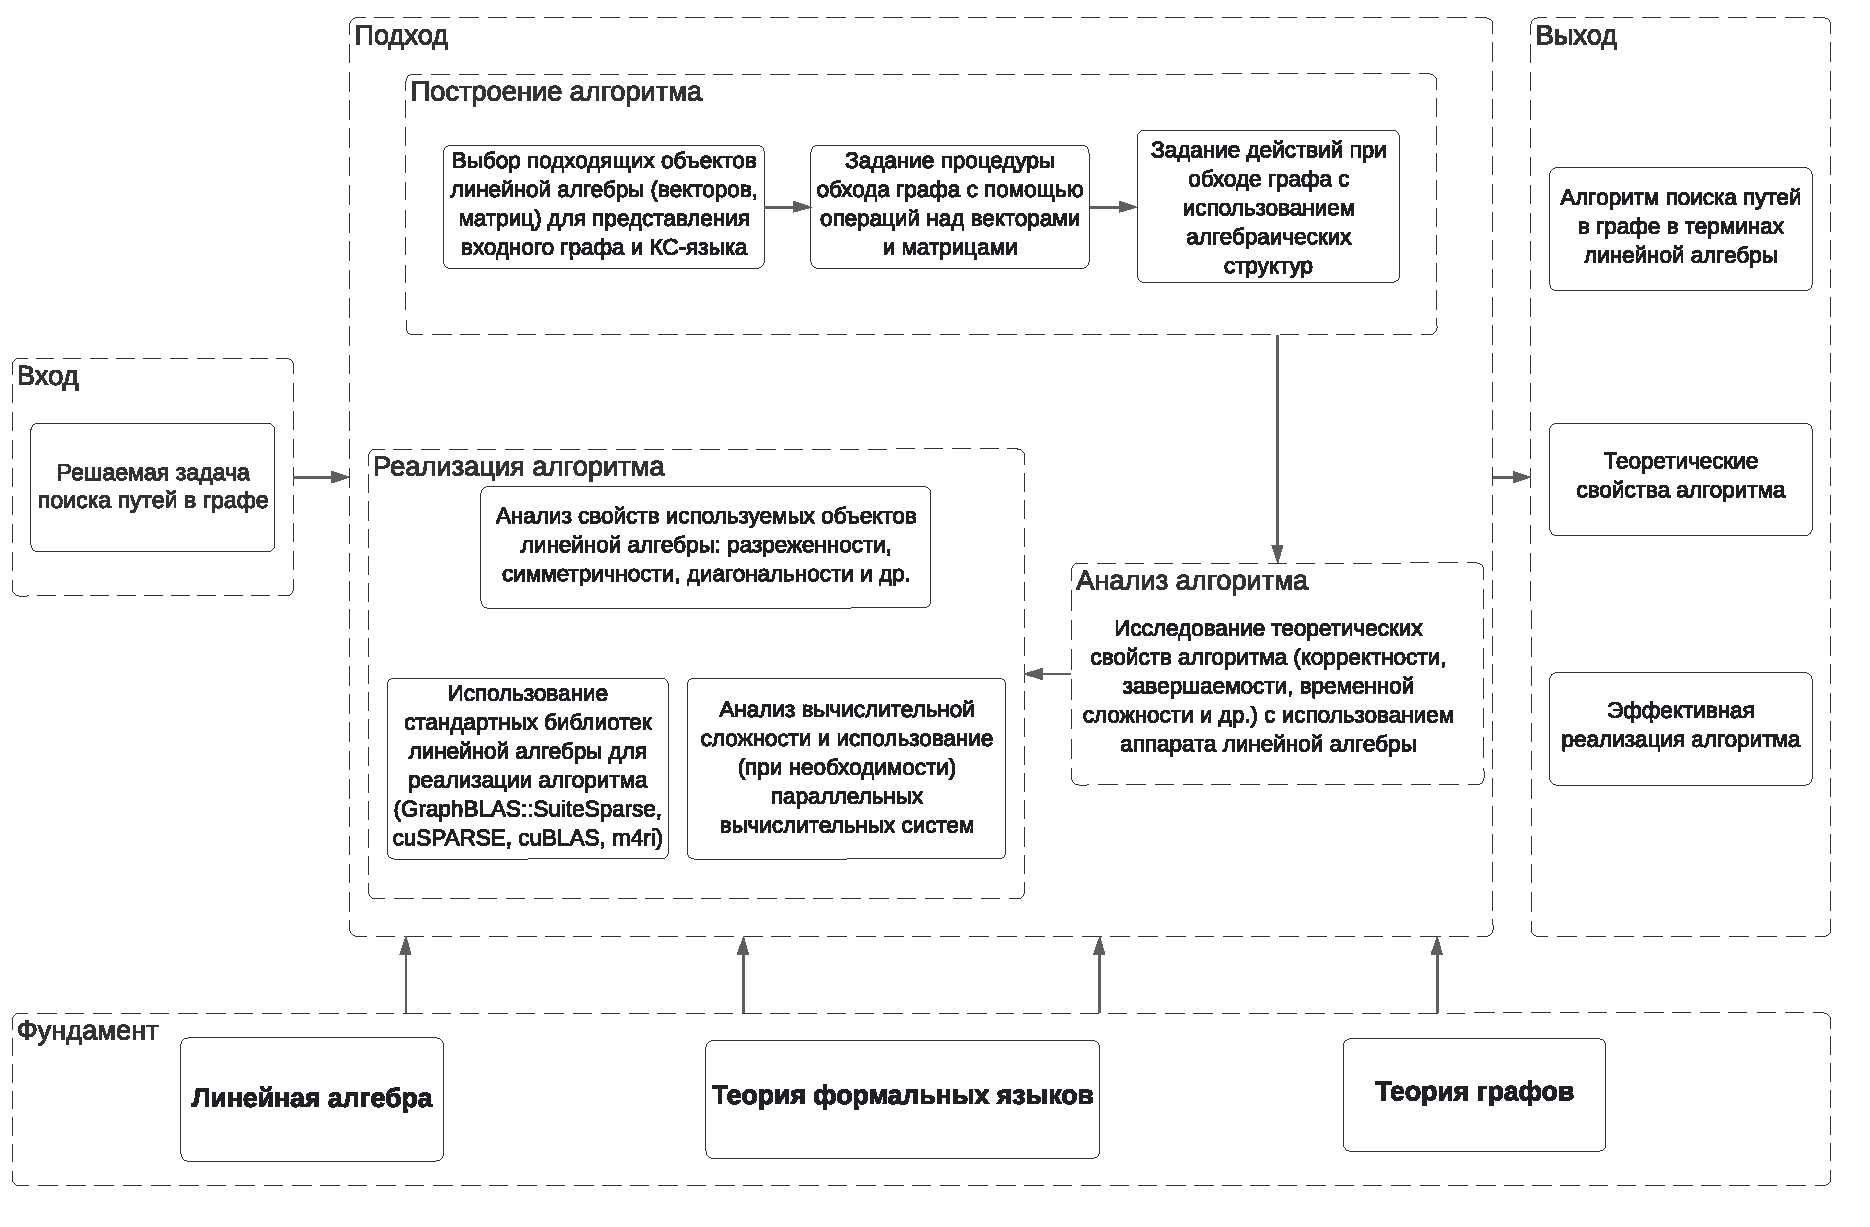
\includegraphics[width = 12cm]{Dissertation/images/schema.pdf}
	\caption{Схема подхода к поиску путей в графе с заданными КС-ограничениями с использованием методов линейной алгебры}
	\label{fig:schema}
\end{figure}

Предлагаемый подход можно разделить на следующие части:
\begin{itemize}
    \item построение алгоритма поиска путей в графе с заданными КС-ограничениями в терминах линейной алгебры;
    \item анализ теоретических свойств построенного алгоритма и поставленной задачи;
    \item реализация построенного алгоритма.
\end{itemize}

Новизна предложенного подхода заключается в следующем.
\begin{enumerate}
    \item Имеющиеся на сегодняшний день подходы к поиску путей в графах с заданными КС-ограничениями либо не используют методы линейной алгебры, либо предназначены только для частного случая КС-ограничений и/или специализированных графов.
    \item Предложенный подход позволяет использовать широкий класс оптимизаций операций линейной алгебры для эффективной работы с графами больших размеров.
    \item Предложенный подход позволяет строить алгоритмы, которые просты в реализации, переносимы, позволяют легко и эффективно использовать параллельные вычисления.
\end{enumerate}


В \underline{\textbf{третьей главе}} изложены алгоритмы поиска путей в графе с заданными КС-ограничениями с использованием матричных операций. Изложенные алгоритмы решают задачи достижимости, поиска одного пути и поиска всех путей в графе с заданными КС-ограничениями. Сформулированы и доказаны утверждения о корректности изложенных алгоритмов. Работа изложенных алгоритмов продемонстрирована на примере. Изложенные алгоритмы реализованы с использованием CPU и GPU-технологий. Проведено экспериментальное исследование разработанных алгоритмов на синтетических и реальных данных.

В \underline{\textbf{четвертой главе}} изложены алгоритмы поиска путей в графе с заданными КС-ограничениями, которые используют операции линейной алгебры, а также не требуют трансформации входной КС-грамматики. Изложенные алгоритмы решают задачи достижимости, поиска одного пути и поиска всех путей в графе с заданными КС-ограничениями. Сформулированы и доказаны утверждения о корректности изложенных алгоритмов. Работа изложенных алгоритмов продемонстрирована на примере. Изложенные алгоритмы реализованы с использованием CPU-технологий. Проведено экспериментальное исследование разработанных алгоритмов на синтетических и реальных данных. Проведено сравнение полученных в диссертации реализаций между собой и с существующими решениями.

В \underline{\textbf{пятой главе}} рассмотрены границы применимости полученных в работе результатов. Представлено сравнение полученных результатов с основными существующими решениями задачи поиска путей в графе с заданными КС-ограничениями.

\FloatBarrier
\pdfbookmark{Заключение}{conclusion}                                  % Закладка pdf
В \underline{\textbf{заключении}} приведены основные результаты работы, которые заключаются в следующем.
%% Согласно ГОСТ Р 7.0.11-2011:
%% 5.3.3 В заключении диссертации излагают итоги выполненного исследования, рекомендации, перспективы дальнейшей разработки темы.
%% 9.2.3 В заключении автореферата диссертации излагают итоги данного исследования, рекомендации и перспективы дальнейшей разработки темы.

\begin{enumerate}[beginpenalty=10000] % https://tex.stackexchange.com/a/476052/104425
	\item Разработан подход к поиску путей в графе с заданными КС-ограничениями на основе методов линейной алгебры, который позволяет использовать теоретические и практические достижения линейной алгебры для решения данной задачи.
	\item Разработан алгоритм, использующий предложенный подход и решающий задачи поиска путей в графе с заданными КС-ограничениями. Доказана завершаемость и корректность предложенного алгоритма. Получена теоретическая оценка сверху временной сложности алгоритма. Предложенный алгоритм использует операции над матрицами, которые позволяют применять широкий класс оптимизаций и дают возможность автоматически распараллеливать вычисления за счёт существующих библиотек линейной алгебры.
	\item Разработан алгоритм поиска путей в графе с заданными КС-ограничениями, использующий предложенный подход и не требующий преобразования входной КС-грамматики. Доказана завершаемость и корректность предложенного алгоритма. Получена теоретическая оценка сверху временной сложности алгоритма. Предложенный алгоритм позволяет работать с произвольными входными КС-грамматиками без необходимости их преобразования, что позволяет избежать значительного увеличения размеров входной грамматики и увлечения времени работы алгоритма.
	\item Предложенные алгоритмы реализованы с использованием параллельных вычислений. Проведено экспериментальное исследование разработанных алгоритмов на реальных RDF данных и графах, построенных для статического анализа программ. Было проведено сравнение полученных реализаций между собой, с существующими решениями из области статического анализа и с решениями, основанными на различных алгоритмах синтаксического анализа. Результаты сравнения показывают, что предложенные реализации для задачи достижимости позволяют ускорить время анализа до 2 порядков и потребляют до 2 раз меньше памяти по сравнению с существующими решениями, а для задач поиска одного и поиска всех путей в графе позволяют ускорить время анализа до 3 порядков и до 2 порядков снизить потребление памяти.
\end{enumerate}


\pdfbookmark{Литература}{bibliography}                                % Закладка pdf

\newcounter{firstbib}

\section*{\bibtitleauthor}
\begin{enumerate}
    \item Azimov R. Context-Free Path Querying by
	Matrix Multiplication / Azimov R., Grigorev S. // In Proceedings of the
	1st Joint International Workshop on Graph Data Management Experiences \&
	Systems (GRADES) and Network Data Analytics (NDA) (GRADES-NDA’18)
	\item Azimov R. Context-Free Path Querying with Single-Path Semantics by
	Matrix Multiplication / Terekhov A., Khoroshev A., Azimov R., Grigorev S. // In Proceedings of the
	3rd Joint International Workshop on Graph Data Management Experiences \&
	Systems (GRADES) and Network Data Analytics (NDA) (GRADES-NDA’20)
	\item Azimov R. Context-Free Path Querying by Kronecker
	Product / Orachev E., Epelbaum I., Azimov R., Grigorev S. // In Proceedings of the
	24th European Conference on Advances in Databases and Information Systems (ADBIS’20)
	\item Azimov R. Context-Free Path Querying with All-Path Semantics by
	Matrix Multiplication / Azimov R., Epelbaum I., Grigorev S. // In Proceedings of the
	4th Joint International Workshop on Graph Data Management Experiences \&
	Systems (GRADES) and Network Data Analytics (NDA) (GRADES-NDA’21)
	
	\item Azimov R. Context-Free Path Querying In Terms of Linear Algebra / Azimov R. // In Proceedings of the VLDB 2021 PhD Workshop (VLDB-PhD'21)
	
	\item Azimov R. Path Querying with Conjunctive Grammars by Matrix Multiplication / Azimov R., Grigorev S. //Programming and Computer Software. – 2019. – Vol. 45. – №. 7. – pp. 357-364.
	\setcounter{firstbib}{\value{enumiv}}
	
	\item Азимов Р. Ш. Синтаксический анализ графов с использованием конъюнктивных грамматик / Азимов Р., Григорьев С. // Труды ИСП РАН, 2018, том 1 вып. 2, с. 3-4.
	\item Азимов Р. Ш. Алгоритм поиска всех путей в графе с заданными контекстно-свободными ограничениями с использованием матриц с множествами промежуточных вершин / Азимов Р., Григорьев С. // Научно-технический вестник информационных технологий, механики и оптики, 2021, том 21, вып. 4, с. 499–505.
\end{enumerate}

\urlstyle{tt}                               % возвращаем установки шрифта ссылок URL
